
% \definecolor{citecolor}{RGB}{34, 149, 34}

\def\httilde{\mbox{\tt\raisebox{-.5ex}{\symbol{126}}}}


\vskip 0.3in


\section*{\LARGE{Appendix}}
\maketitle


\section{Ablation on Interpolation Radius}
In the main paper, we use a default radius of $r=7$ when interpolating masked-out features (Eqn.~\ref{eqn:lambda} and following text). Here we demonstrate that the radius of 7 is reasonable through an ablation experiment, whose results are listed in Table~\ref{tab:radius}. The experiment is conducted with HRNet-W18 on Cityscapes semantic segmentation, with both redesigned head (RH) and confidence adaptivity (CA). We observe that a radius of 7 outperforms lower ones (3 and 5) in the average mIoU slightly, with minimal FLOPs addition, due to the fact that interpolation is done channel-wise. A further increase of radius to 9 does not bring significant gain in final or average mIoU.
\begin{table}[h]
\vspace{0ex}
\centering
\footnotesize
\begin{tabular}{cc|ccccc|ccccc}
\hline
\multicolumn{2}{c|}{}                            & \multicolumn{5}{c}{Accuracy (mIoU)}         & \multicolumn{5}{|c}{Computation (GFLOPs)}            \\ \hline
\multicolumn{2}{c|}{Radius}             & 1    & 2    & 3    & 4    & Avg  & 1     & 2     & 3     & 4      & Avg   \\ \hline
& 3 & 41.06 &	48.25 &	67.56 &	75.82  & 58.17  &  23.7 &  33.0 & 44.4 & 57.0 &   39.5  \\ 
& 5 & 40.86 &	48.01 &	67.64 &	76.21  & 58.18  &  23.7 & 33.1 & 44.6 & 57.4 &   39.7  \\ 
& 7 (default) & 41.05 &	48.35 &	67.73 &	76.10  & 58.31  & 23.7 & 33.1 & 44.9 & 58.1 &   40.0  \\ 
& 9 & 41.01 &	48.41 &	67.88 &	76.08 & 58.35  &  23.7 & 33.2 & 45.4 & 59.1 &   40.4  \\  \hline
\end{tabular}
\vspace{0ex}
\caption{%
Accuracy (mIoU) and inference computation (GFLOPs) for Cityscapes semantic segmentation with four exits under different settings of interpolation radius. A minor increase in mIoU and GFLOPs is observed with a larger radius.
}
\vspace{-1ex}
\label{tab:radius}
\end{table}

\section{Inference-Only Confidence Adaptivity}
\begin{table}[h]
\vspace{0ex}
\centering
\footnotesize
\begin{tabular}{cc|ccccc|ccccc}
\hline
\multicolumn{2}{c|}{}                            & \multicolumn{5}{c}{Accuracy (mIoU)}         & \multicolumn{5}{|c}{Computation (GFLOPs)}            \\ \hline
\multicolumn{2}{c|}{Adaptivity}             & 1    & 2    & 3    & 4    & Avg  & 1     & 2     & 3     & 4      & Avg   \\ \hline
& No Adaptivity & 44.61  & 60.19 &  76.64  & 79.89 & 65.33   &   41.9 & 105.6 & 368.0 & 701.4 & 304.2  \\ 
& Training and Inference & 44.34 &	60.13 &	76.82 &	81.31  & 65.65 & 41.9 & 93.9 & 259.4 & 387.1 & 195.6  \\ 
& Inference-only & 44.61 &  59.97 &  76.37 &  79.69 & 65.16     & 41.9 &  94.1 &  291.8 & 484.8 & 228.1  \\ \hline
\end{tabular}
\vspace{0ex}
\caption{%
Accuracy (mIoU) and inference computation (GFLOPs) for Cityscapes semantic segmentation with four exits under different adaptivity settings.
}
\vspace{-1ex}
\label{tab:inference-only}
\end{table}

In the experiment section of the main paper, confidence adaptivity is used in both training and inference. Here we compare this with the setting where adaptivity is only used for inference in Table~\ref{tab:inference-only}. We use HRNet-W48 with redesigned heads (RH) on Cityscapes for this experiment. ``No Adaptivity'' corresponds to the ``EE + RH'' row in Table~\ref{tab:semseg}. We observe that using adaptivity only at inference hurts the accuracy, compared with using it at both training and inference. It also increases the average FLOPs at exit 3 and 4.



\section{Experimental Settings}
\label{app:train}
For Cityscapes semantic segmentation, we follow the training settings at the official codebase \cite{hrnet_ss_github} of HRNet for semantic segmentation. The HRNet-W18/48 models are pre-trained on ImageNet. During training, multi-scale and flipping data augmentation is used, and the input cropping size is $512\times 1024$. The model is trained for 484 epochs, with an initial learning rate of 0.01 and a polynomial schedule of power 0.9, a weight decay of 0.0005, a batch size of 12, optimized by SGD with 0.9 momentum. In evaluation, we use single-scale testing without flipping, with input resolution $1024\times 2048$. For the Feature-Based Stochastic Sampling baseline, we modify the exit weights from $(1, 1, 1, 1)$ to $(0.5, 0.5, 0.5, 1)$ as we find it produces more stable masking values during training. The $L_1$ sparsity regularization on masks is set to $0.1$. The mask outputs at exit $(1,2,3)$ have additional weight factors of $(1/3, 2/3, 1)$ to encourage more sparse features towards the end.

For MPII human pose estimation, we follow the training settings at the official codebase \cite{hrnet_hpe_github} of HRNet for pose estimation. The HRNet-32 model we use is also pre-trained on ImageNet. The image size for both training and evaluation is $256\times 256$. The model is trained for 210 epochs, with an initial learning rate of 0.001, and decaying of 0.1 at epoch 170 and 200. The optimization is done by Adam with $\gamma_1=0.99, \gamma_2=0$, a weight decay of 0.0001, and a momentum of 0.9. The batch size is 128. In evaluation, flipping test is used.

% \clearpage
\section{PASCAL-Context Results}
We present results with the PASCAL-Context semantic segmentation dataset \cite{mottaghi_cvpr14} in Table~\ref{tab:pascal}. It consists of 59 segmentation classes.
For the Early Exiting baseline, we use weights of (0.33, 0.33, 0.33, 1) for 4 exits, respectively, as we found increasing it to all 1 would hurt the final performance too much. 
The confidence threshold is set to 99.5\%. We observe RH improve the accuracy in most exits. ADP-C outperforms the Early Exiting baseline in average mIoU, despite its final mIoU is worse. It also saves more than 20\% FLOPs compared with the vanilla Early Exiting baseline.

\setlength{\tabcolsep}{2pt}
\renewcommand{\arraystretch}{1.2}
\begin{table}[h]
\vspace{0ex}
\centering
\footnotesize
\begin{tabular}{c|l|ccccc|ccccc}
\hline
\multicolumn{2}{c|}{}                              & \multicolumn{5}{c}{Accuracy (mIoU)}         & \multicolumn{5}{|c}{Computation (GFLOPs)}            \\ \hline
\multicolumn{2}{c|}{Method / Output}               & 1    & 2    & 3    & 4    & Avg  & 1     & 2     & 3     & 4      & Avg   \\ \hline
 One-exit & HRNet-W48 \cite{wang2020deep}          & -    & -    & -    & 51.35 & -    & -     & -     & -     & 76.5  & -     \\ \hline
\multirow{1}{*}{Baseline} & Early Exiting (HRNet) & 8.78 & 18.74 & 39.82 & 50.10 & 29.36 & 5.4  &12.6 & 43.1 & 80.1  & 35.3 \\
                           \hline
\multirow{2}{*}{Ours}      
                           & EE + RH (HRNet)      & 14.55 & 19.42 & 39.30 & 50.32 & 30.90 & 4.5 & 11.4  & 40.2 & 77.2  & 33.3 \\
                           & ADP-C: EE + RH + CA (HRNet) & 14.51 & 19.18 & 39.00 & 49.27 & 30.49 & 4.5 & 11.1  & 38.1 & \textbf{62.7}  & 29.1 \\ \hline
\end{tabular}
\vspace{0ex}
\caption{%
Accuracy (mIoU) and inference computation (GFLOPs) for PASCAL-Context semantic segmentation. 
}
\vspace{-1ex}
\label{tab:pascal}
\end{table}


\section{More Visualizations}
\label{app:vis}

\begin{figure}[H]
% \vspace{-1ex}
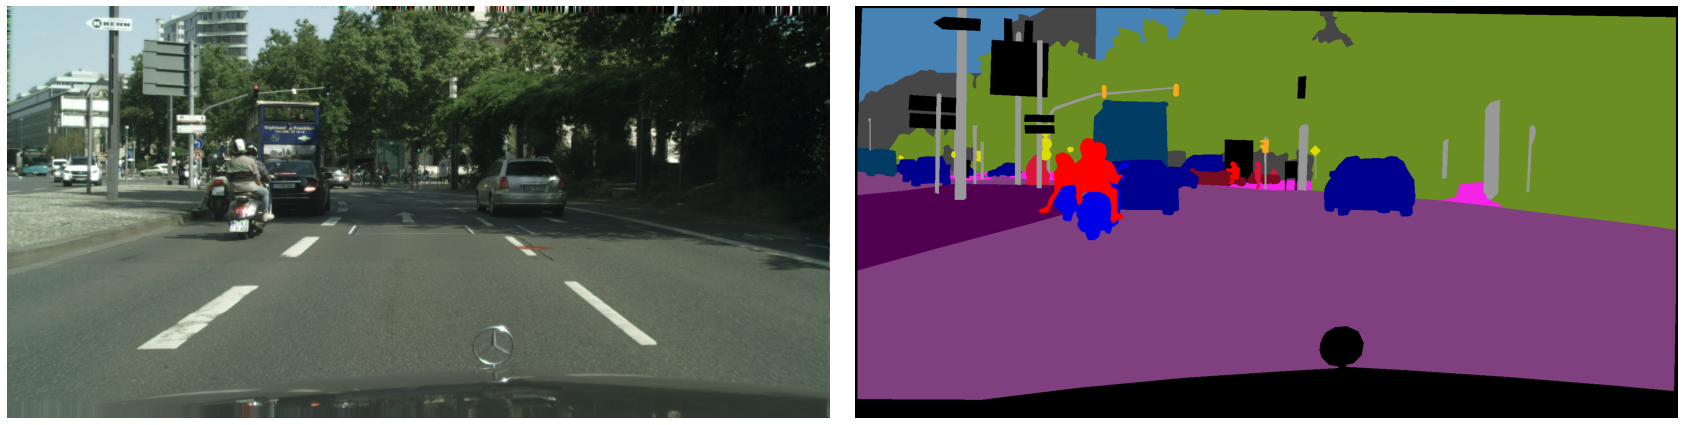
\includegraphics[width=.50\textwidth]{images/vis_supp/input_gt_frankfurt_000000_017476.png}
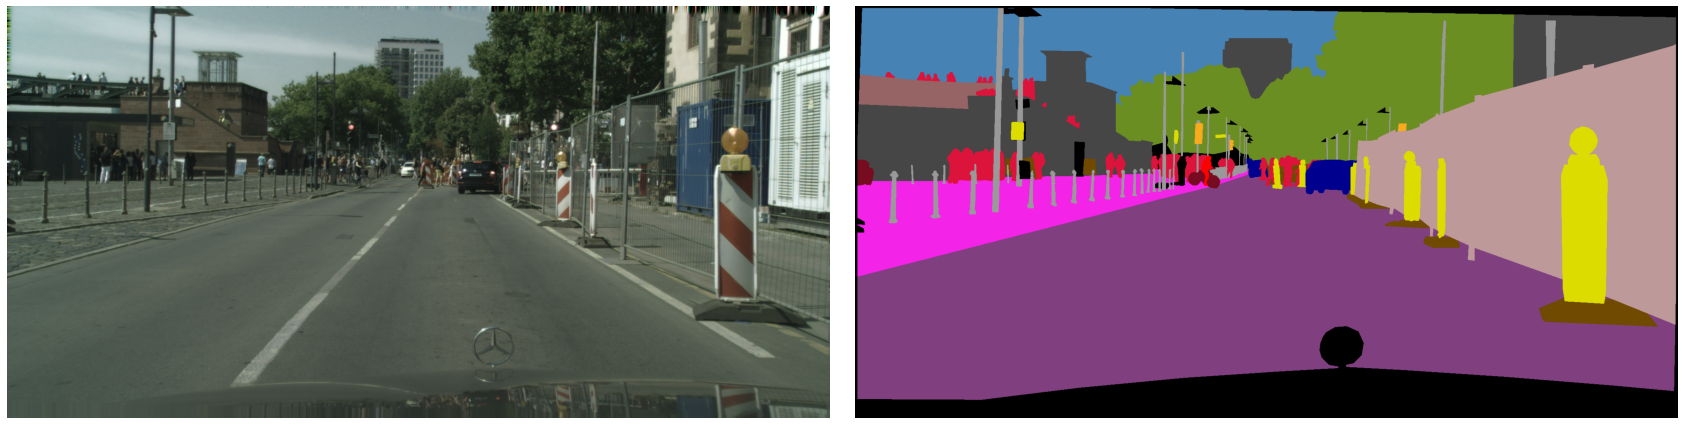
\includegraphics[width=.50\textwidth]{images/vis_supp/input_gt_frankfurt_000001_005184.png}
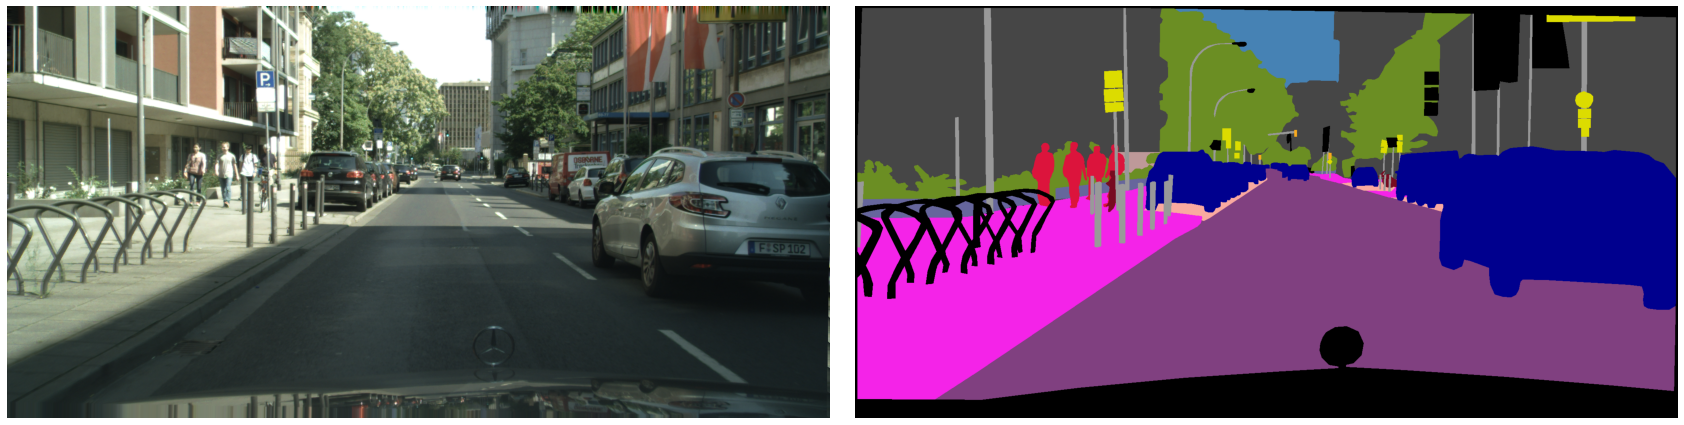
\includegraphics[width=.50\textwidth]{images/vis_supp/input_gt_frankfurt_000001_028335.png}
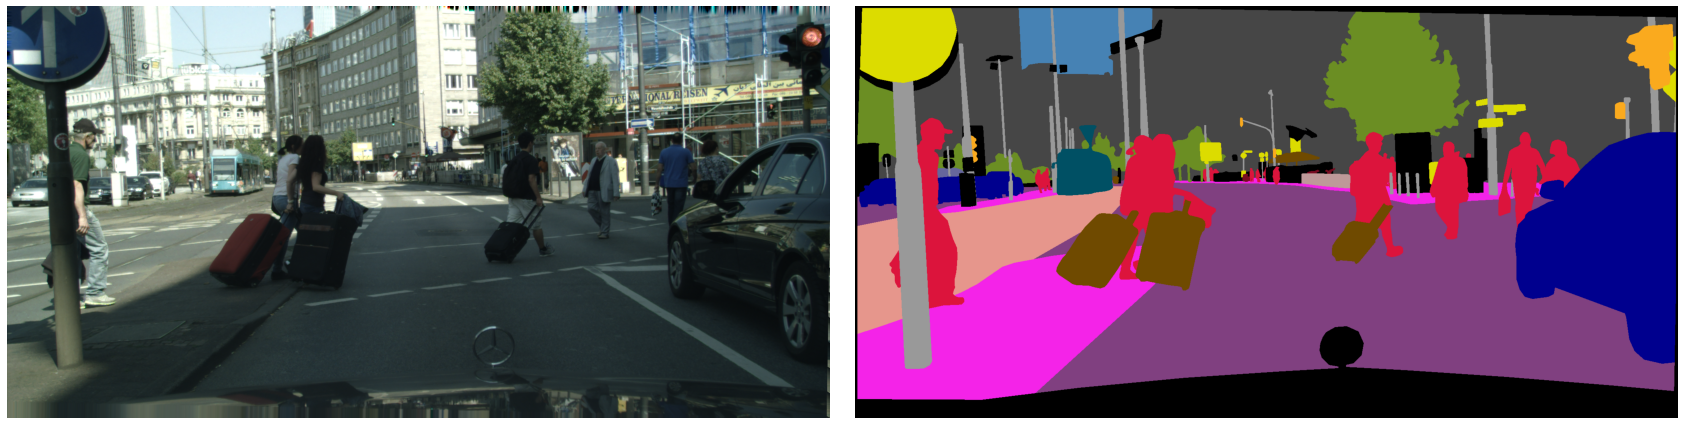
\includegraphics[width=.50\textwidth]{images/vis_supp/input_gt_frankfurt_000001_037705.png}
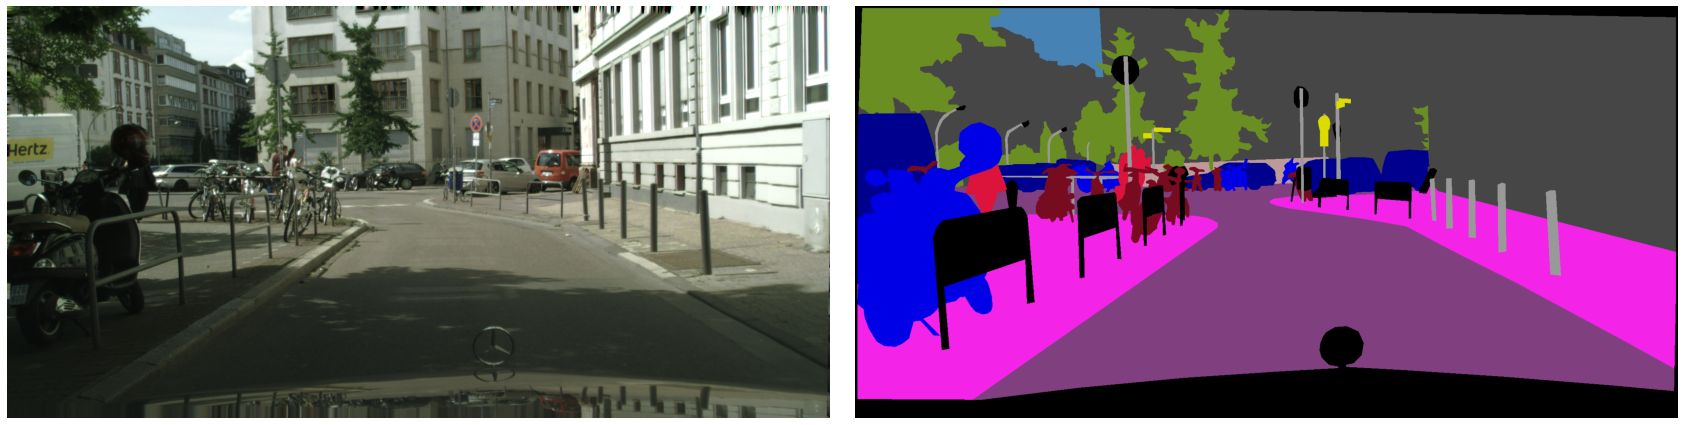
\includegraphics[width=.50\textwidth]{images/vis_supp/input_gt_frankfurt_000001_064130.png}
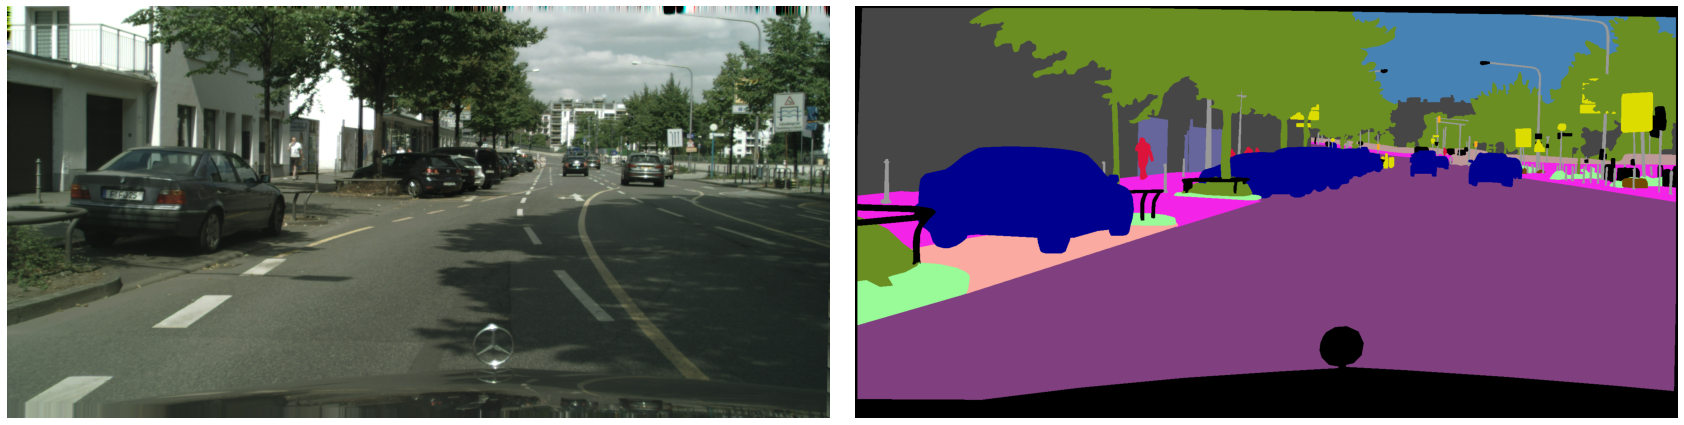
\includegraphics[width=.50\textwidth]{images/vis_supp/input_gt_frankfurt_000001_080391.png}
\vspace{-4ex}
\caption{Input and ground truth of the example validation images visualized in Fig.~\ref{fig:vis1} and Fig.~\ref{fig:vis2}}
\label{fig:gt}
\end{figure}
\vspace{-2ex}
We present more visualizations of the same type as Fig.~\ref{fig:vis} in the main paper, in Fig.~\ref{fig:vis1} and \ref{fig:vis2}. Their input and ground truth are shown in Fig.~\ref{fig:gt} in the same order. We can see the same trend as discussed in the main paper still holds: the model will mask out confident points that are inside large segments (e.g., road, vegetable), which are mostly already predicted correctly in early exits.

\begin{figure*}[htbp]
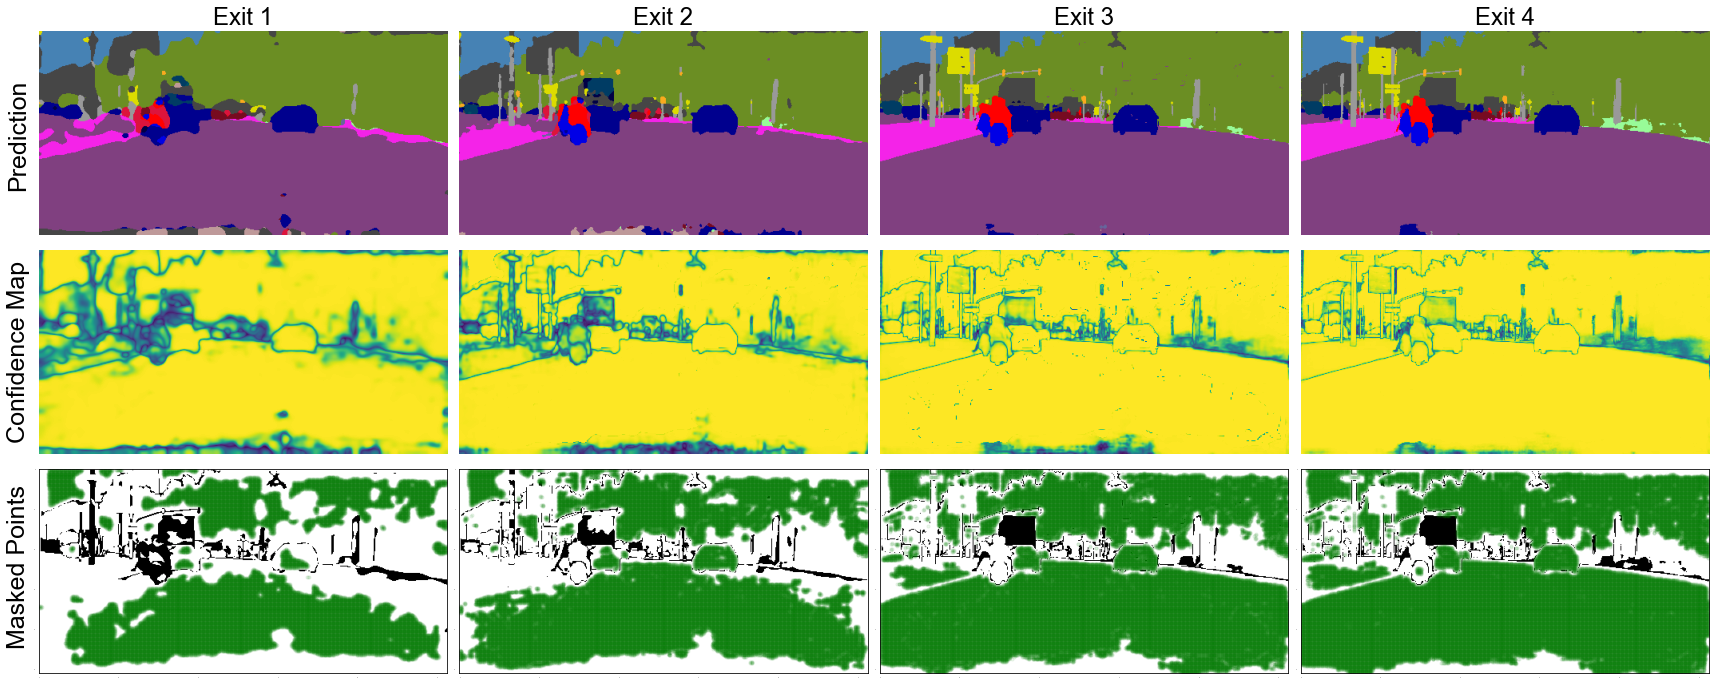
\includegraphics[width=\textwidth]{images/vis_supp/visualize_final_frankfurt_000000_017476.png}
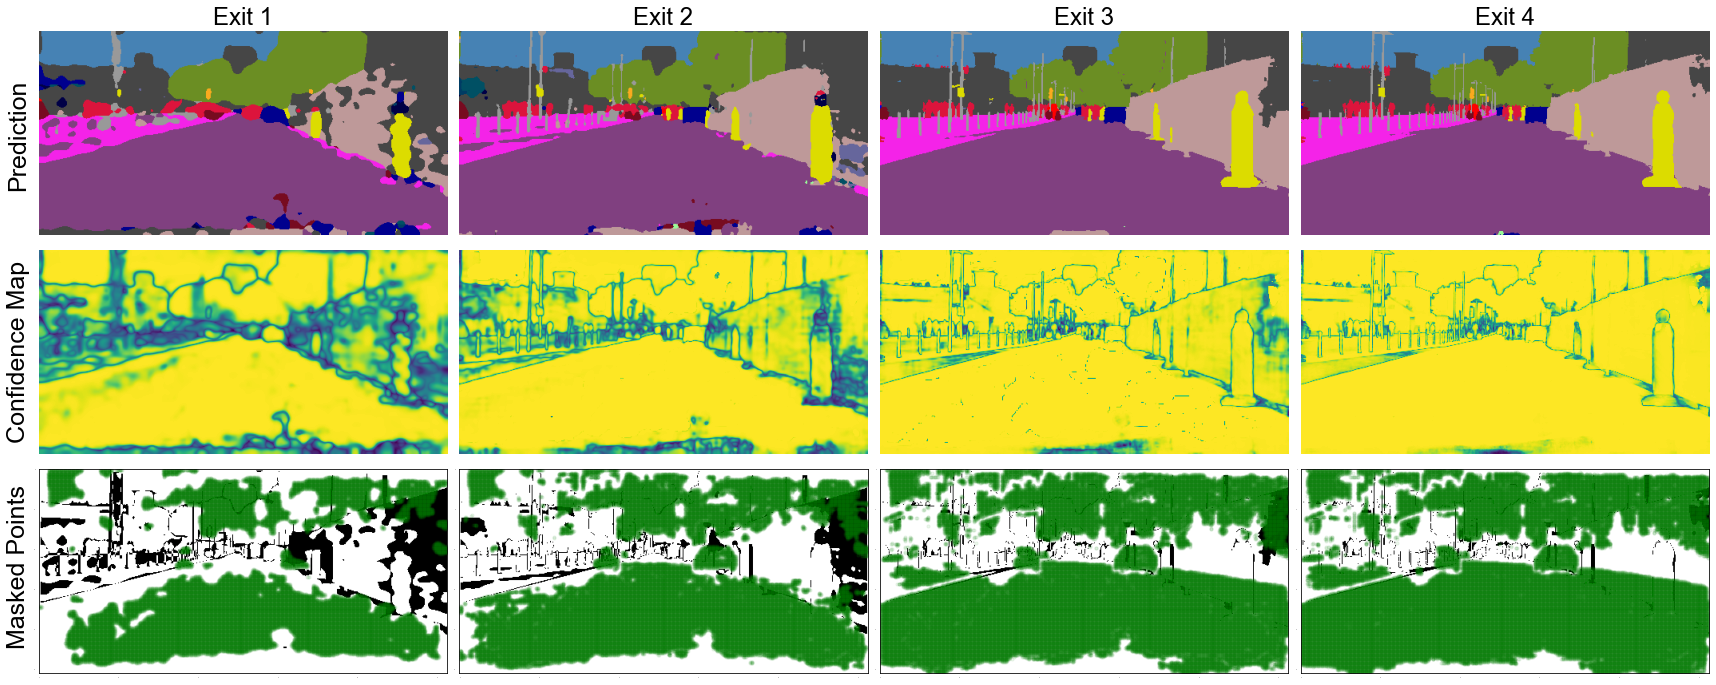
\includegraphics[width=\textwidth]{images/vis_supp/visualize_final_frankfurt_000001_005184.png}
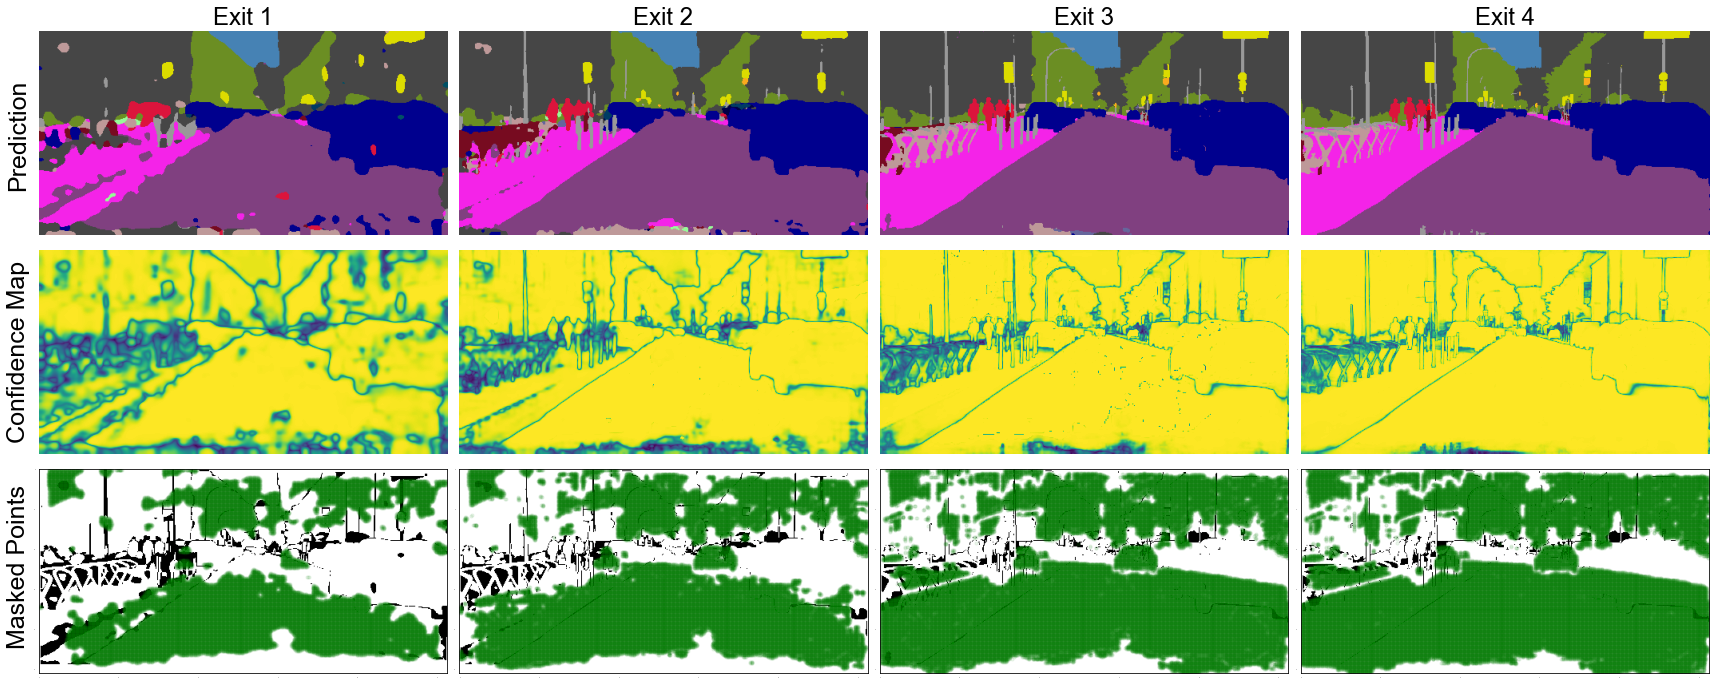
\includegraphics[width=\textwidth]{images/vis_supp/visualize_final_frankfurt_000001_028335.png}
\caption{%
Top: prediction results at all exits.
Middle: confidence maps, lighter color (yellow) indicates higher confidence.
Bottom: correct/wrong predictions at the exit drawn as white/black.
The confident points selected for masking are in green.
Confidence adaptivity excludes calculation on already confident pixels (green) in early exits, mostly located at inner parts of large segments.}
\label{fig:vis1}
\end{figure*}

\begin{figure*}[htbp]
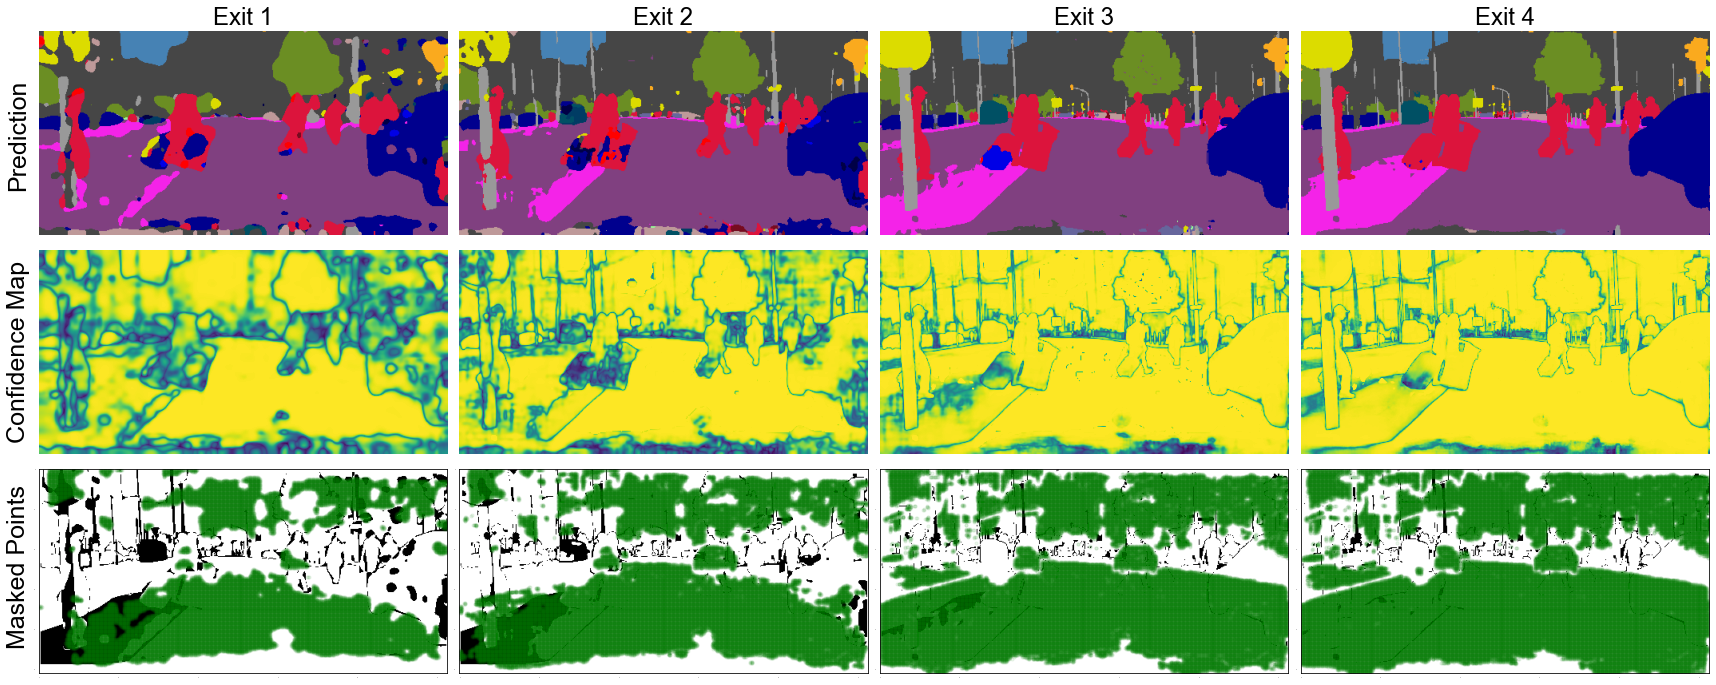
\includegraphics[width=\textwidth]{images/vis_supp/visualize_final_frankfurt_000001_037705.png}
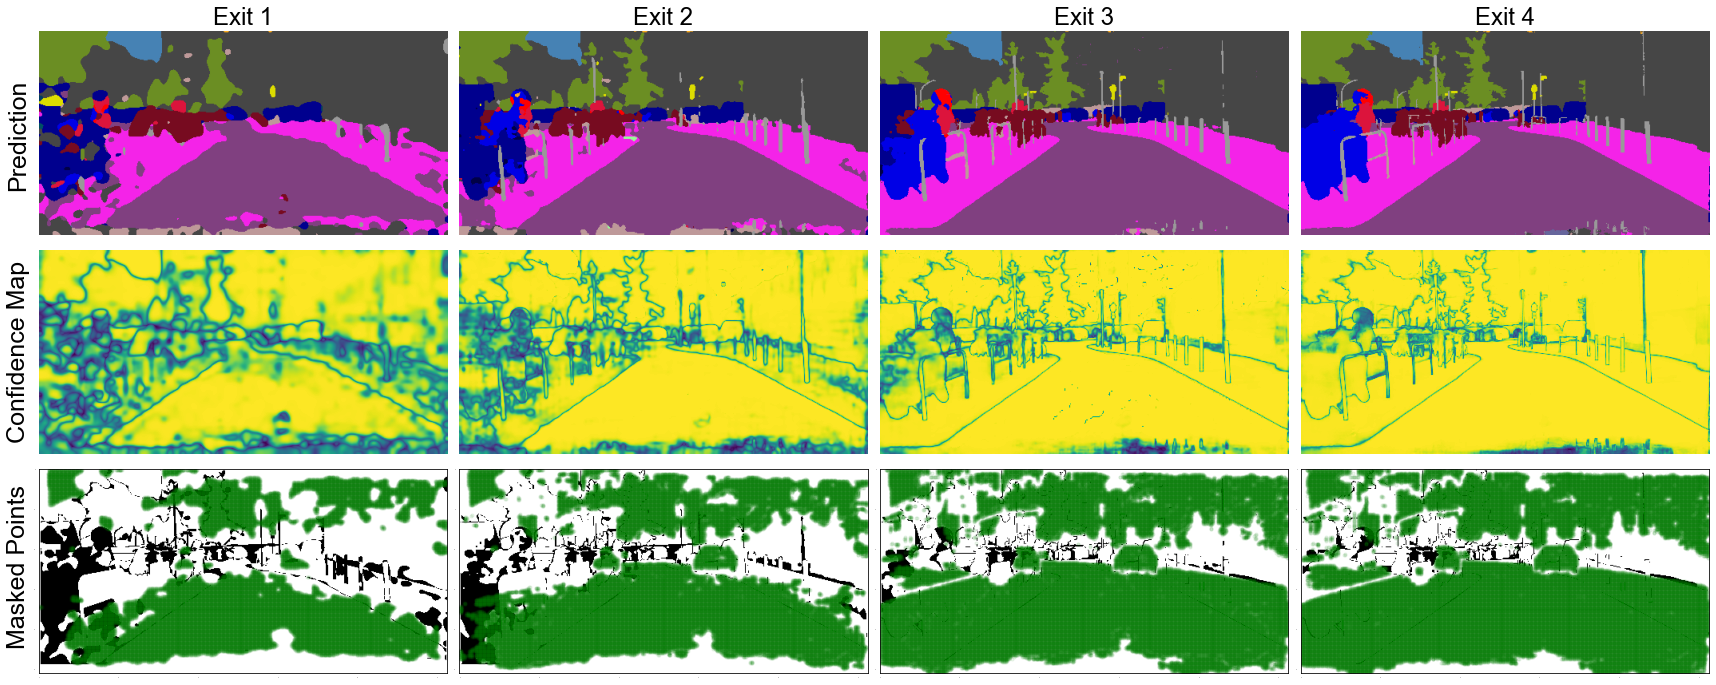
\includegraphics[width=\textwidth]{images/vis_supp/visualize_final_frankfurt_000001_064130.png}
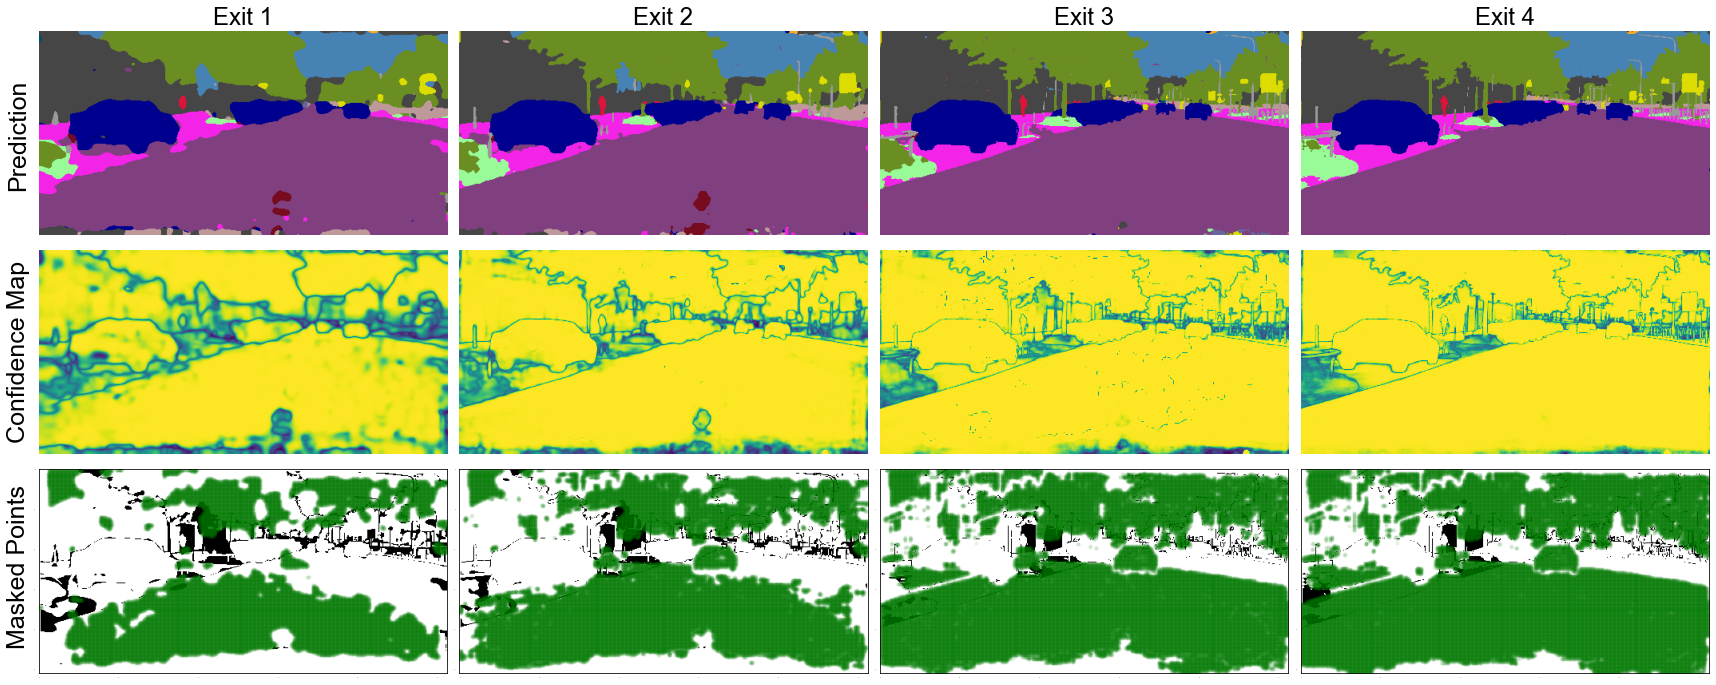
\includegraphics[width=\textwidth]{images/vis_supp/visualize_final_frankfurt_000001_080391.png}
\caption{%
Top: prediction results at all exits.
Middle: confidence maps, lighter color (yellow) indicates higher confidence.
Bottom: correct/wrong predictions at the exit drawn as white/black.
The confident points selected for masking are in green.
Confidence adaptivity excludes calculation on already confident pixels (green) in early exits, mostly located at inner parts of large segments.}
\vspace{-2ex}
\label{fig:vis2}
\end{figure*}

\clearpage


% \section{More MDEQ Results}
% \label{app:mdeq}
% In the main paper, we used MDEQ's ``small'' model's 4th, 6th, 8th, and 10th iterations' results to align with our model's 4 exits. In this section, we provide full results on Cityscapes semantic segmentation at all iterations for both the ``small'' and the ``XL'' (extra-large) models at Table \ref{tab:mdeq_full}. The original configuration \cite{mdeq} sets the number of iterations to 26 and 27 for MDEQ-small and MDEQ-XL. In Fig. \ref{fig:mdeq_vis1} and \ref{fig:mdeq_vis2}, we also provide qualitative visualization of results for the same 6 validation images from Fig. \ref{fig:gt}, with MDEQ-small at 4th, 6th, 8th, 10th, 14th, 18th, 22th, 26th iterations. With the progression of iterations, the predictions get more and more accurate.

% % \begin{table*}[htbp]
% \setlength{\tabcolsep}{4pt}
% \renewcommand{\arraystretch}{1.1}
% \begin{table}[h]
% \centering
% \small
% \begin{tabular}{c|cc|cc}
% \hline
%                         & \multicolumn{2}{c|}{MDEQ-Small} & \multicolumn{2}{c}{MDEQ-XL} \\ \hline
% Iteration         & mIoU                & GFLOPs                & mIoU                & GFLOPs                \\ \hline
% 1 & 1.1  & 227.2  &    1.9 &   1983.0  \\ 
% 2 & 1.1  & 325.3  &    1.9 &   2861.3  \\ 
% 3 & 9.0  & 423.5  &    8.0 &   3739.6  \\ 
% 4 & 17.3 & 521.6  &    11.6 &   4617.9  \\ 
% 5 & 38.7 & 619.7  &    34.1 &   5496.2  \\ 
% 6 & 38.7 & 717.9  &    49.4 &   6374.5  \\ 
% 7 & 61.0 & 816.0  &    58.6 &   7252.9  \\ 
% 8 & 65.5 & 914.2  &    67.1 &   8131.2  \\ 
% 9 & 70.1 & 1012.3 &    71.6 &   9009.5  \\ 
% 10 & 72.4 & 1110.5 &    74.5 &   9887.8  \\ 
% 11 & 73.8 & 1208.5 &    76.1 &   10766.1 \\ 
% 12 & 74.6 & 1306.7 &    77.3 &   11644.4 \\ 
% 13 & 75.1 & 1404.8 &    77.9 &   12522.7 \\ 
% 14 & 75.5 & 1503.0 &    78.7 &   13401.0 \\ 
% 15 & 75.8 & 1601.1 &    79.1 &   14279.3 \\ 
% 16 & 75.9 & 1699.3 &    79.3 &   15157.6 \\ 
% 17 & 76.1 & 1797.4 &    79.5 &   16036.0 \\ 
% 18 & 76.2 & 1895.5 &    79.6 &   16914.3 \\ 
% 19 & 76.2 & 1993.7 &    79.6 &   17792.6 \\ 
% 20 & 76.2 & 2091.8 &    79.7 &   18670.9 \\ 
% 21 & 76.2 & 2190.0 &    79.8 &   19549.2 \\ 
% 22 & 76.1 & 2288.1 &    79.9 &   20427.5 \\ 
% 23 & 76.2 & 2386.2 &    79.9 &   21305.8 \\ 
% 24 & 76.3 & 2484.4 &    79.9 &   22184.2 \\ 
% 25 & 76.4 & 2582.5 &    79.9 &   23062.5 \\ 
% 26 & 76.5 & 2680.7 &    79.8 &   23940.8 \\ 
% 27 & 76.5 & 2778.8 &    79.8 &   24819.1 \\ \hline
% \end{tabular}
% \vspace{2ex}
% \caption{%
% Accuracy (mIoU) and computation (GFLOPs) on Cityscapes semantic segmentation for MDEQ models, at different iterations.}

% \label{tab:mdeq_full}
% \end{table}

% \begin{figure*}[htbp]
% 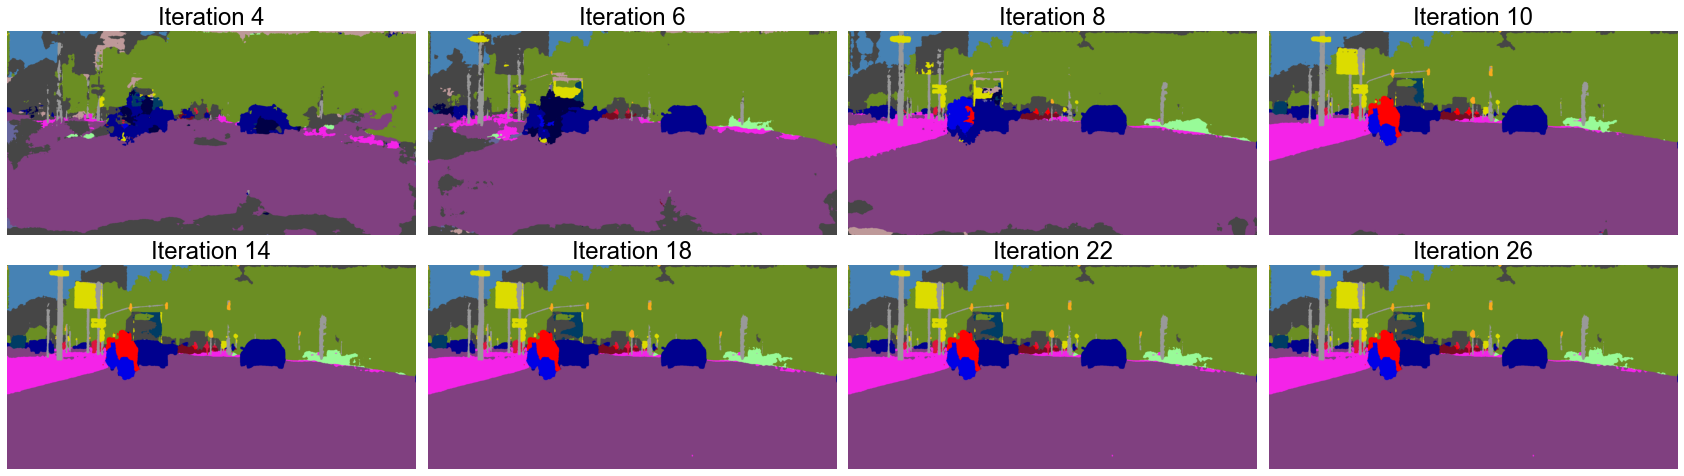
\includegraphics[width=\textwidth]{images/vis_supp/mdeq/visualize_final_frankfurt_000000_017476.png}
% \vspace{1ex}
% 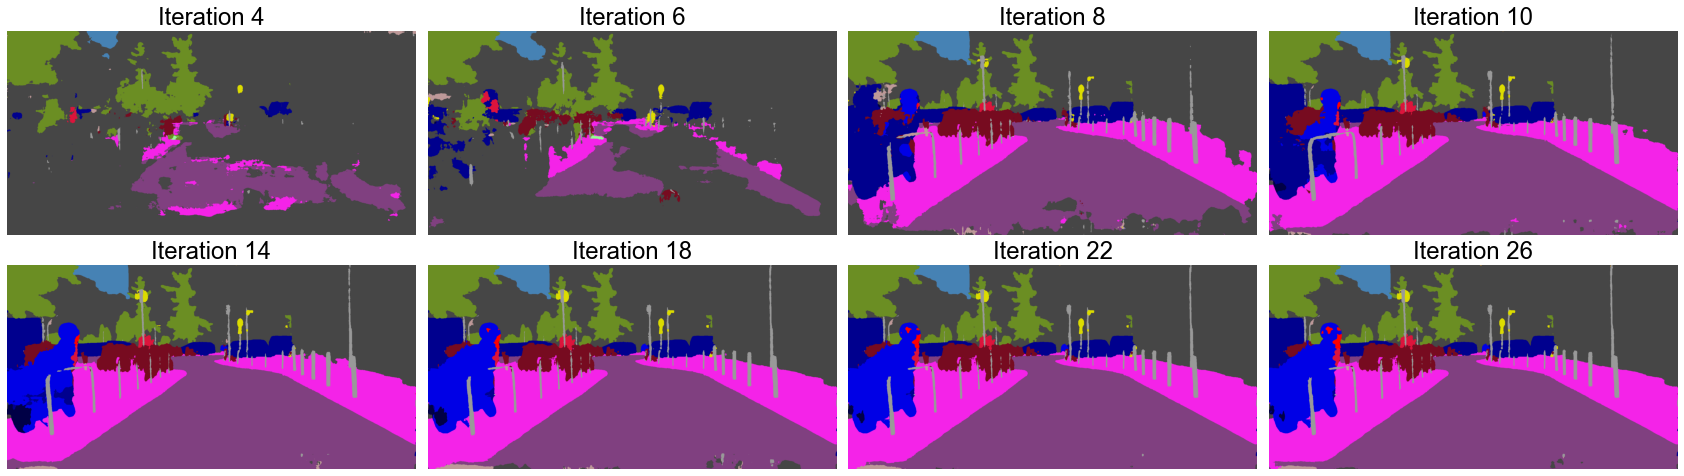
\includegraphics[width=\textwidth]{images/vis_supp/mdeq/visualize_final_frankfurt_000001_064130.png}
% \vspace{1ex}
% 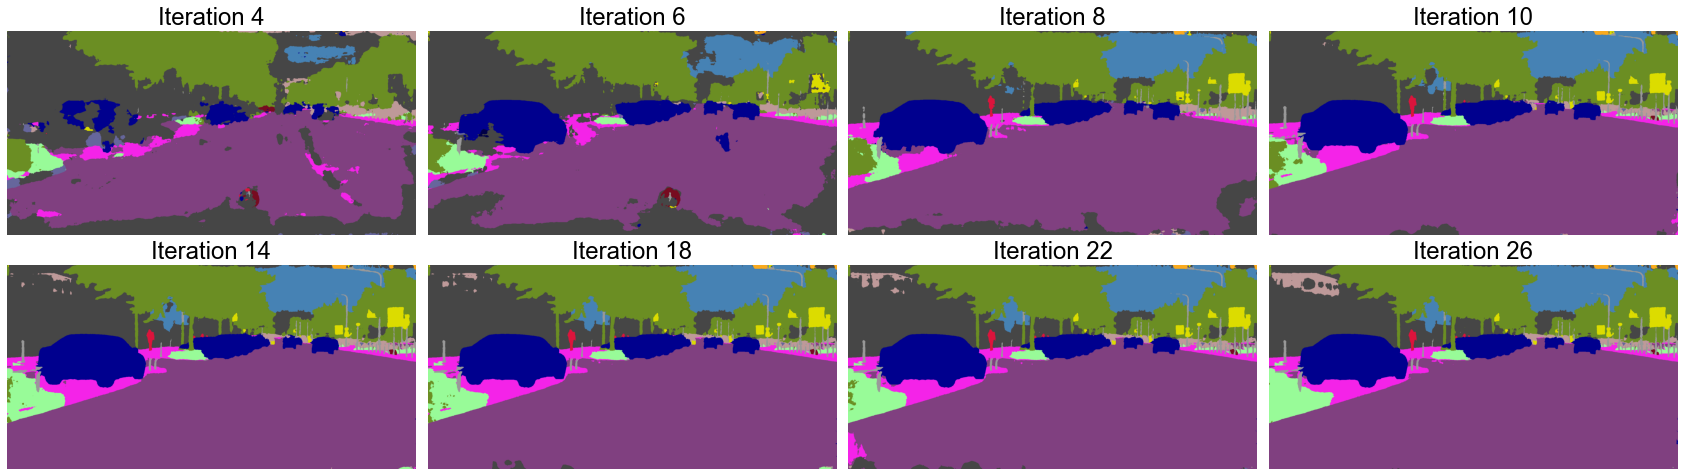
\includegraphics[width=\textwidth]{images/vis_supp/mdeq/visualize_final_frankfurt_000001_080391.png}
% \caption{%
% Cityscapes prediction results for MDEQ-Small all various iterations. Input and ground truth are in Fig. \ref{fig:gt}.}
% \label{fig:mdeq_vis1}
% \end{figure*}

% \begin{figure*}[htbp]
% 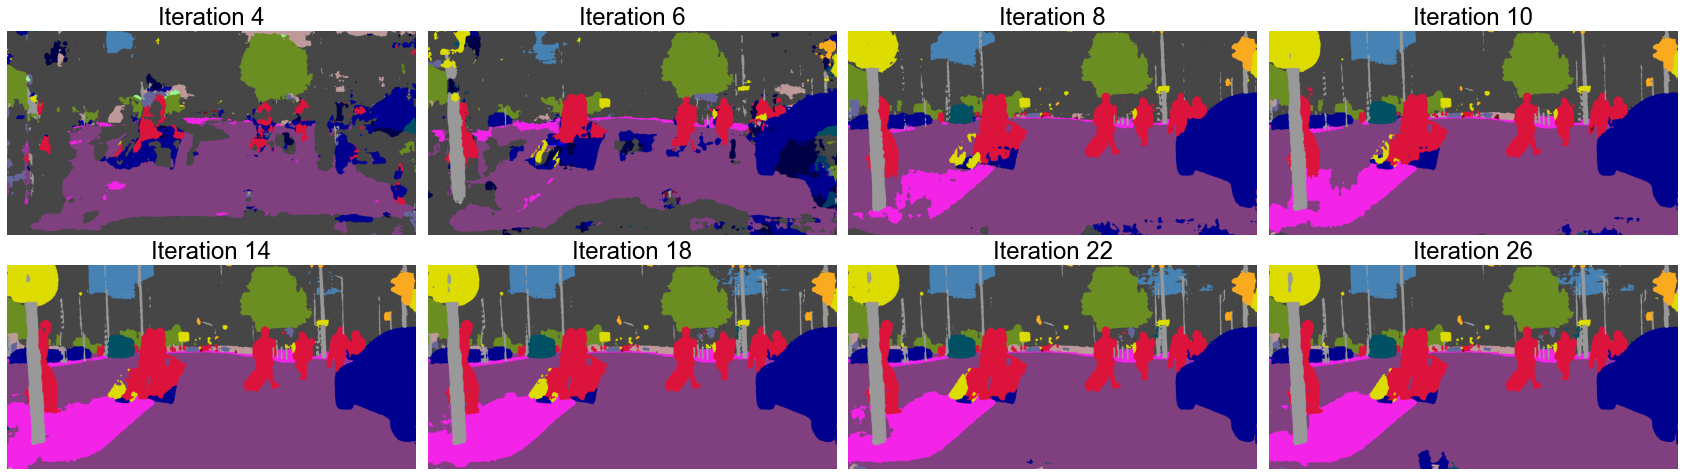
\includegraphics[width=\textwidth]{images/vis_supp/mdeq/visualize_final_frankfurt_000001_037705.png}
% \vspace{1ex}
% 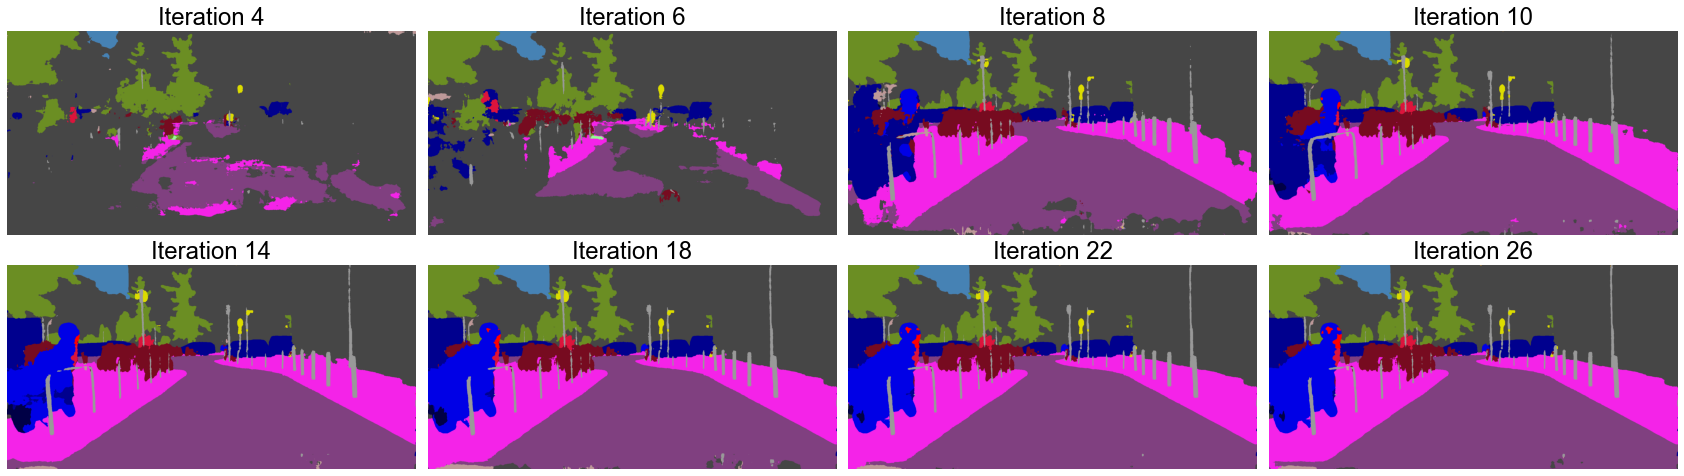
\includegraphics[width=\textwidth]{images/vis_supp/mdeq/visualize_final_frankfurt_000001_064130.png}
% \vspace{1ex}
% 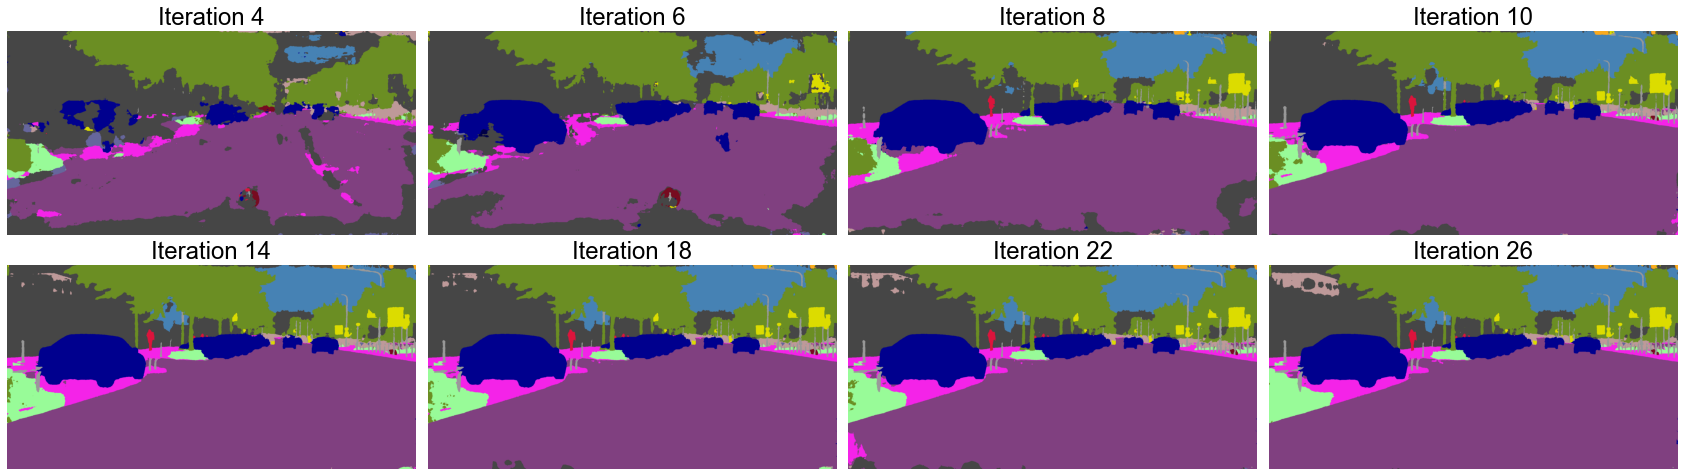
\includegraphics[width=\textwidth]{images/vis_supp/mdeq/visualize_final_frankfurt_000001_080391.png}
% \caption{%
% Cityscapes prediction results for MDEQ-Small all various iterations. Input and ground truth are in Fig. \ref{fig:gt}.}
% \label{fig:mdeq_vis2}
% \end{figure*}





